\documentclass[12pt, a4paper]{article}

\usepackage[margin=2.5cm]{geometry}
\usepackage{graphicx}
\usepackage{amsmath}
\usepackage{amssymb}
\usepackage{booktabs}
\usepackage{hyperref}
\usepackage{listings}
\usepackage{xcolor}
\usepackage{caption}
\usepackage{subcaption}
\usepackage{parskip}
\usepackage{titlesec}
\usepackage{fancyhdr}

\hypersetup{
    colorlinks=true,
    linkcolor=blue!60!black,
    urlcolor=blue!60!black,
}

\lstset{
    language=Python,
    basicstyle=\ttfamily\small,
    keywordstyle=\color{blue!70!black}\bfseries,
    commentstyle=\color{gray},
    stringstyle=\color{orange!80!black},
    breaklines=true,
    frame=single,
    backgroundcolor=\color{gray!8},
    numbers=left,
    numberstyle=\tiny\color{gray},
    xleftmargin=1.5em,
    framexleftmargin=1.5em,
}

\pagestyle{fancy}
\fancyhf{}
\rhead{Collective Robotics -- Tutorial 1}
\lhead{Gandhi, Machida}
\cfoot{\thepage}

\title{
    \vspace{-1cm}
    \textbf{Collective Robotics -- Tutorial 1}\\[0.3em]
    \large Scalability and Synchronization\\[0.5em]
    \normalsize Hochschule Bonn-Rhein-Sieg\\
    Prof.\ Dr.\ Javad Ghofrani
}
\author{Bhavesh Gandhi \and Jaqueline Machida}
\date{17.05.2026}

\begin{document}

\maketitle
\thispagestyle{fancy}
\tableofcontents
\newpage

% =============================================================================
\section{Task 1 -- Scaling of a Computer System}
% =============================================================================

\subsection{Overview}

We model a computer job queue using a Poisson arrival process.
New jobs arrive at rate $\alpha$ per time step; since we set $\Delta t = 1$,
the parameter becomes $\lambda = \alpha$.
The probability that exactly $i$ jobs arrive in one time step is:

\begin{equation}
    P(X = i) = \frac{e^{-\lambda}\,\lambda^{i}}{i!}, \qquad \lambda = \alpha \Delta t = \alpha.
\end{equation}

The server processes jobs one at a time, each taking a fixed number of steps
(the \emph{processing duration}).  We are interested in how the average waiting
queue length depends on $\alpha$.

\subsection{Implementation}

All core logic lives in \texttt{task\_1/queue\_model.py} and is shared by all
subtask scripts.

\paragraph{Poisson PMF (\texttt{poisson\_pmf}).}
Evaluates Equation~(1) analytically using Python's \texttt{math} module.

\paragraph{Sampler (\texttt{sample\_poisson}).}
Draws samples using inverse transform sampling directly from the PMF
in Equation~(1).
A uniform random number $u \in [0,1)$ is drawn and the cumulative probability
$\sum_{k=0}^{i} P(X=k)$ is accumulated until it first exceeds $u$; the
corresponding $i$ is returned as the sample.

\begin{lstlisting}
def sample_poisson(alpha):
    u = random.random()
    cumulative = 0.0
    i = 0
    while True:
        cumulative += poisson_pmf(i, alpha)
        if u < cumulative:
            return i
        i += 1
\end{lstlisting}

\paragraph{Queue simulation (\texttt{simulate\_queue}).}
Each of the $N$ time steps proceeds in two phases:
\begin{enumerate}
    \item \textbf{Arrival phase:} sample the number of new jobs and add them to
          the queue.
    \item \textbf{Processing phase:} if the server is busy, decrement its
          remaining work counter; otherwise, if the queue is non-empty, dequeue
          one job and start processing it for \texttt{processing\_duration} steps.
\end{enumerate}
The function returns the time-average queue length.

\subsection{Subtask a -- Poisson PMF}

Figure~\ref{fig:1a} shows $P(X=i)$ for $\alpha \in \{0.01, 0.1, 0.5, 1\}$.
For very small $\alpha$ the mass is concentrated near $i=0$ (almost no jobs
arrive per step).  As $\alpha$ increases the distribution spreads and its mode
shifts to the right, as expected from a Poisson distribution whose mean and
variance both equal $\lambda = \alpha$.

\begin{figure}[h]
    \centering
    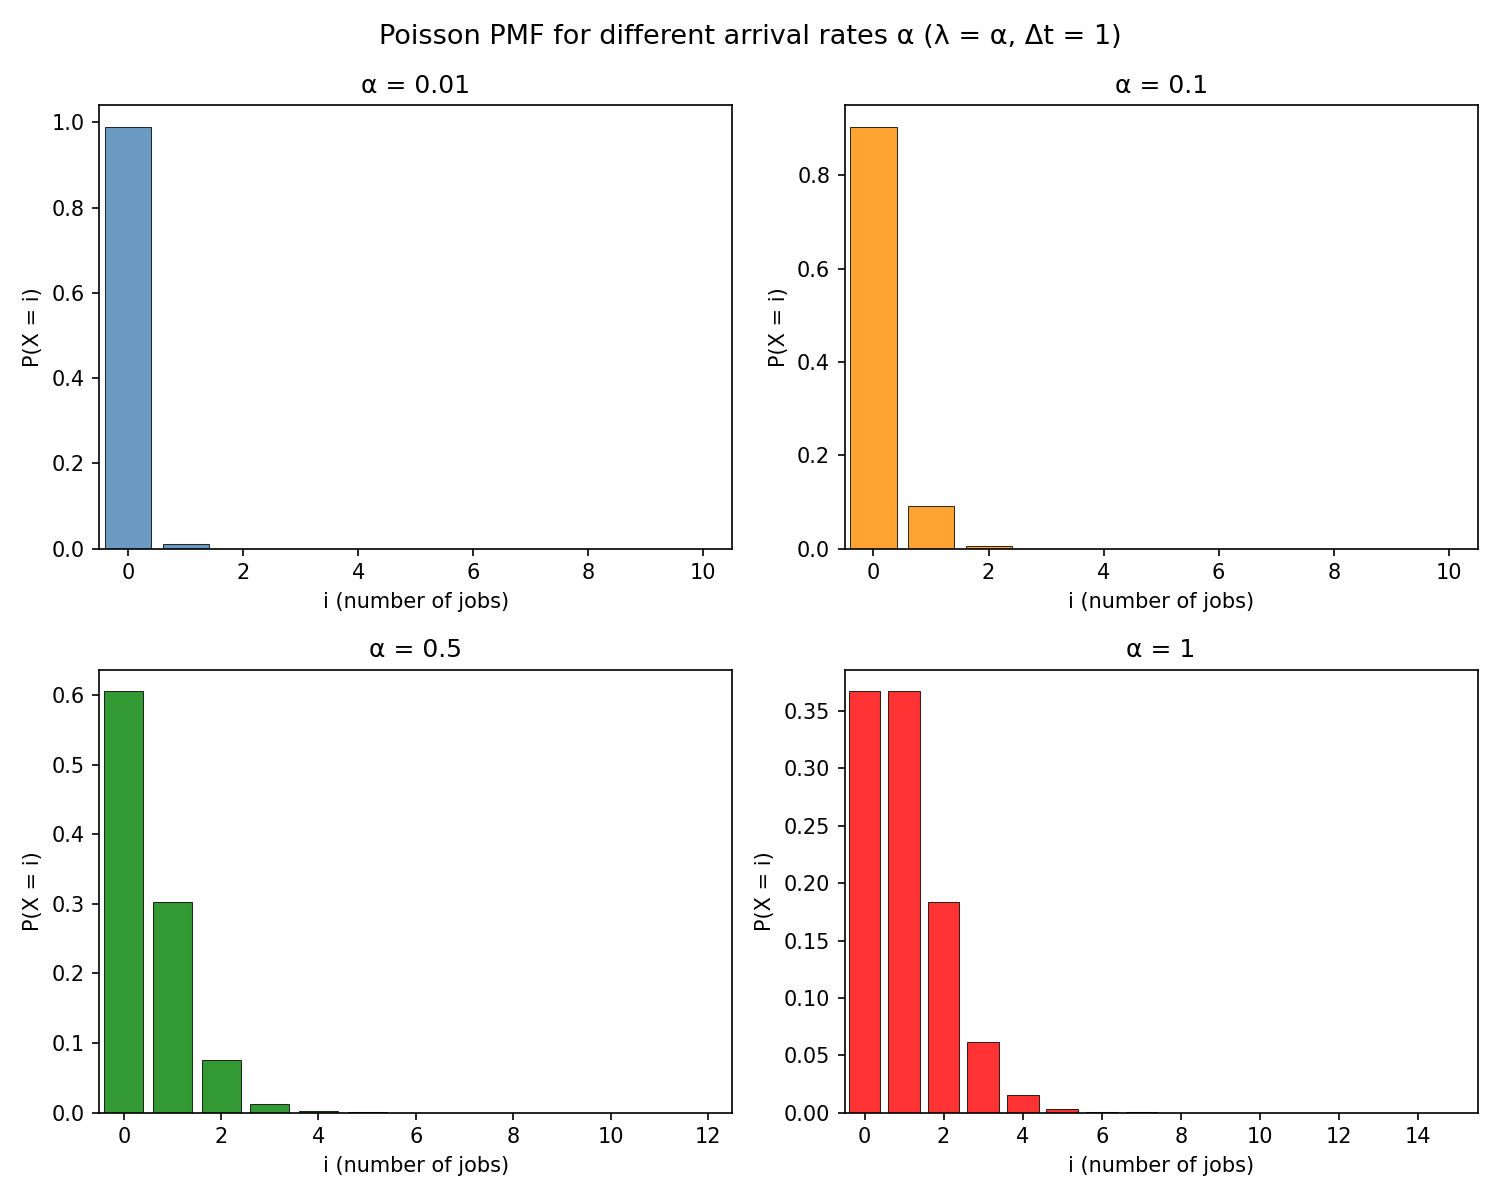
\includegraphics[width=\textwidth]{task_1/plots/task1a_poisson_pmf.png}
    \caption{Poisson PMF $P(X=i)$ for four arrival rates $\alpha$.}
    \label{fig:1a}
\end{figure}

\subsection{Subtask b -- Sampling}

Figure~\ref{fig:1b} compares 10\,000 samples drawn with \texttt{sample\_poisson}
($\alpha = 0.5$) against the analytical PMF.
The empirical bars closely match the theoretical curve, confirming that the
sampler is correct.

\begin{figure}[h]
    \centering
    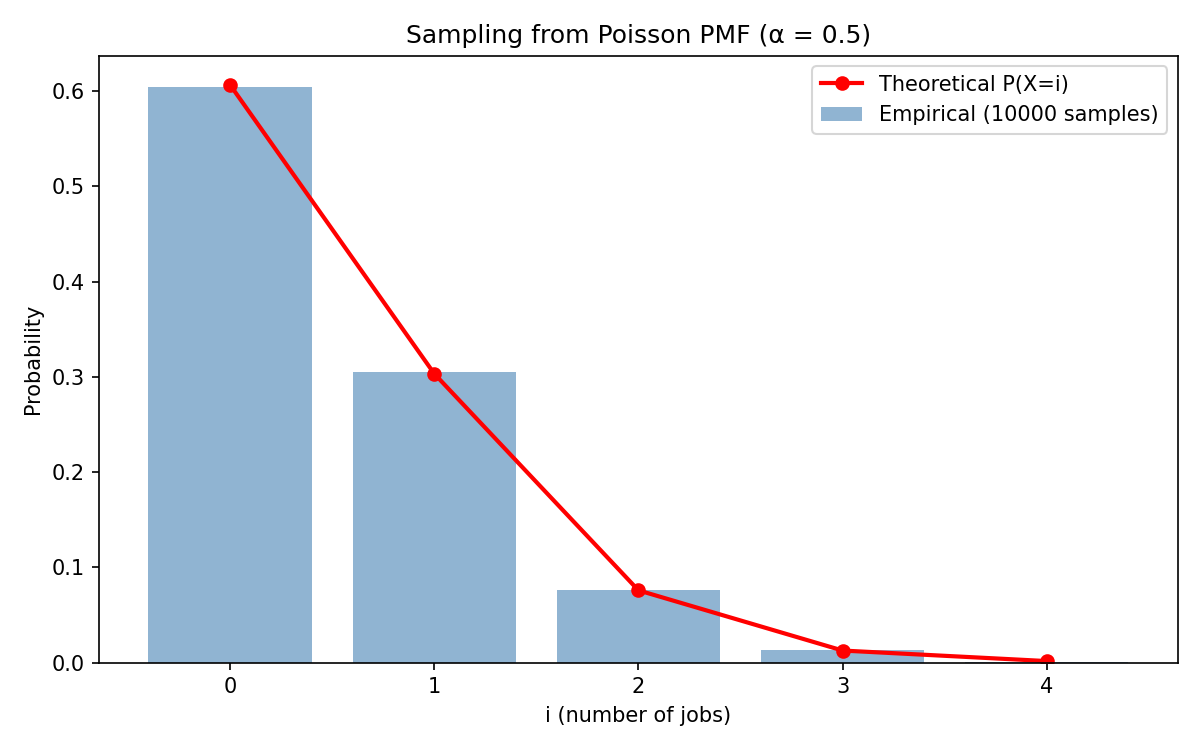
\includegraphics[width=0.75\textwidth]{task_1/plots/task1b_sampling.png}
    \caption{Empirical frequency vs.\ theoretical PMF for $\alpha = 0.5$,
             10\,000 samples.}
    \label{fig:1b}
\end{figure}

\subsection{Subtask c -- Single Simulation Run}

We ran the queue model for 2000 time steps with $\alpha = 0.1$ and a processing
duration of 4 steps per job.  The resulting average queue length was
0.1235 jobs.

This low value is expected: the average arrival rate is $\alpha = 0.1$ jobs/step,
while the server can process $1/4 = 0.25$ jobs/step, so the system is well below
saturation and jobs are rarely queued.

\subsection{Subtask d -- Average Queue Length vs.\ $\alpha$ (4 steps/job)}

We swept $\alpha \in [0.005,\,0.25]$ in steps of $0.005$.  For each value we
ran 200 independent 2000-step simulations and averaged the resulting queue
lengths to obtain one representative point per $\alpha$ (see Figure~\ref{fig:1d}).

\begin{figure}[h]
    \centering
    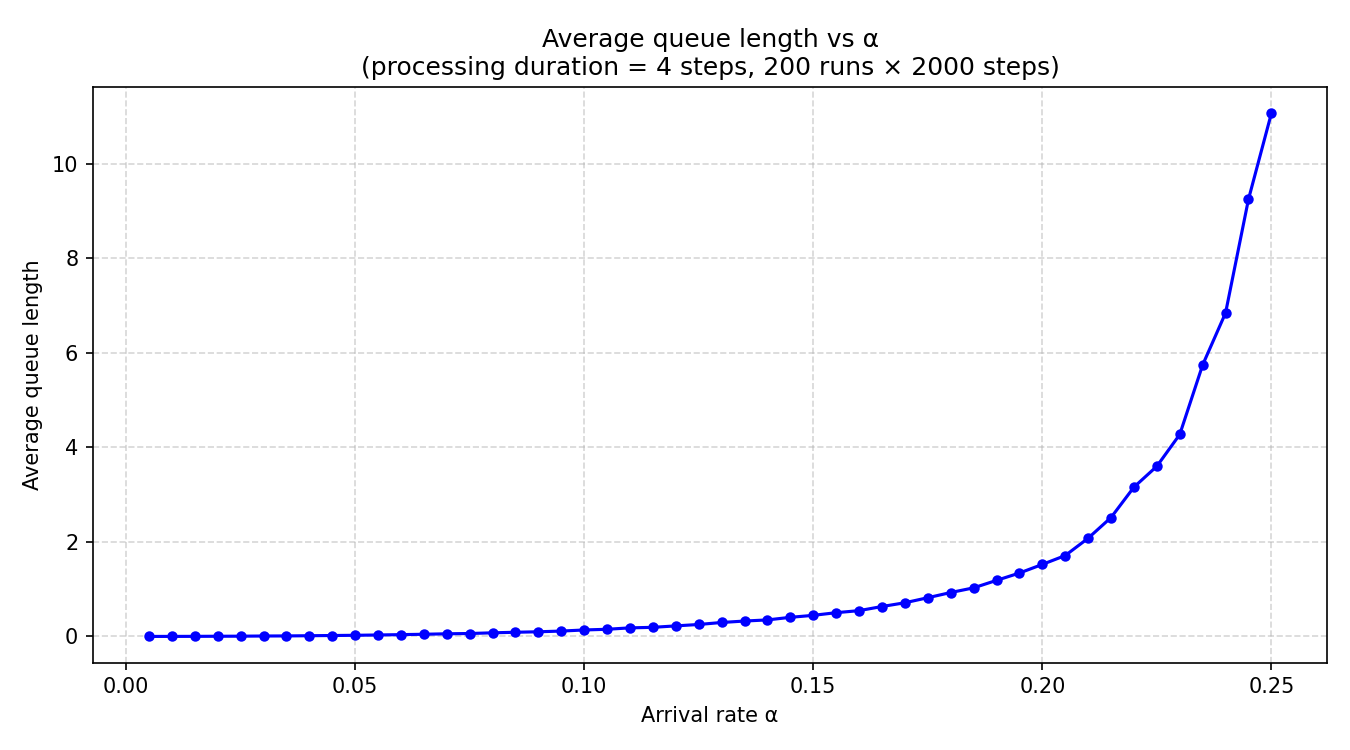
\includegraphics[width=0.85\textwidth]{task_1/plots/task1d_avg_queue_4steps.png}
    \caption{Average queue length as a function of $\alpha$ for a processing
             duration of 4 steps per job (200 runs $\times$ 2000 steps each).}
    \label{fig:1d}
\end{figure}

\paragraph{Discussion.}
The curve is nearly flat and close to zero for small $\alpha$, then rises steeply
as $\alpha$ approaches $0.25$.  This is a classic queuing-theory result: the
system is stable when the arrival rate is below the service rate
($\alpha < 1/\text{processing\_duration} = 0.25$), and the queue diverges as
$\alpha$ approaches $0.25$.

\subsection{Subtask e -- Comparison: 2 vs.\ 4 Steps per Job}

Figure~\ref{fig:1e} shows the same experiment for a processing duration of
2 steps/job with $\alpha \in [0.005,\,0.5]$ alongside the 4-step case.

\begin{figure}[h]
    \centering
    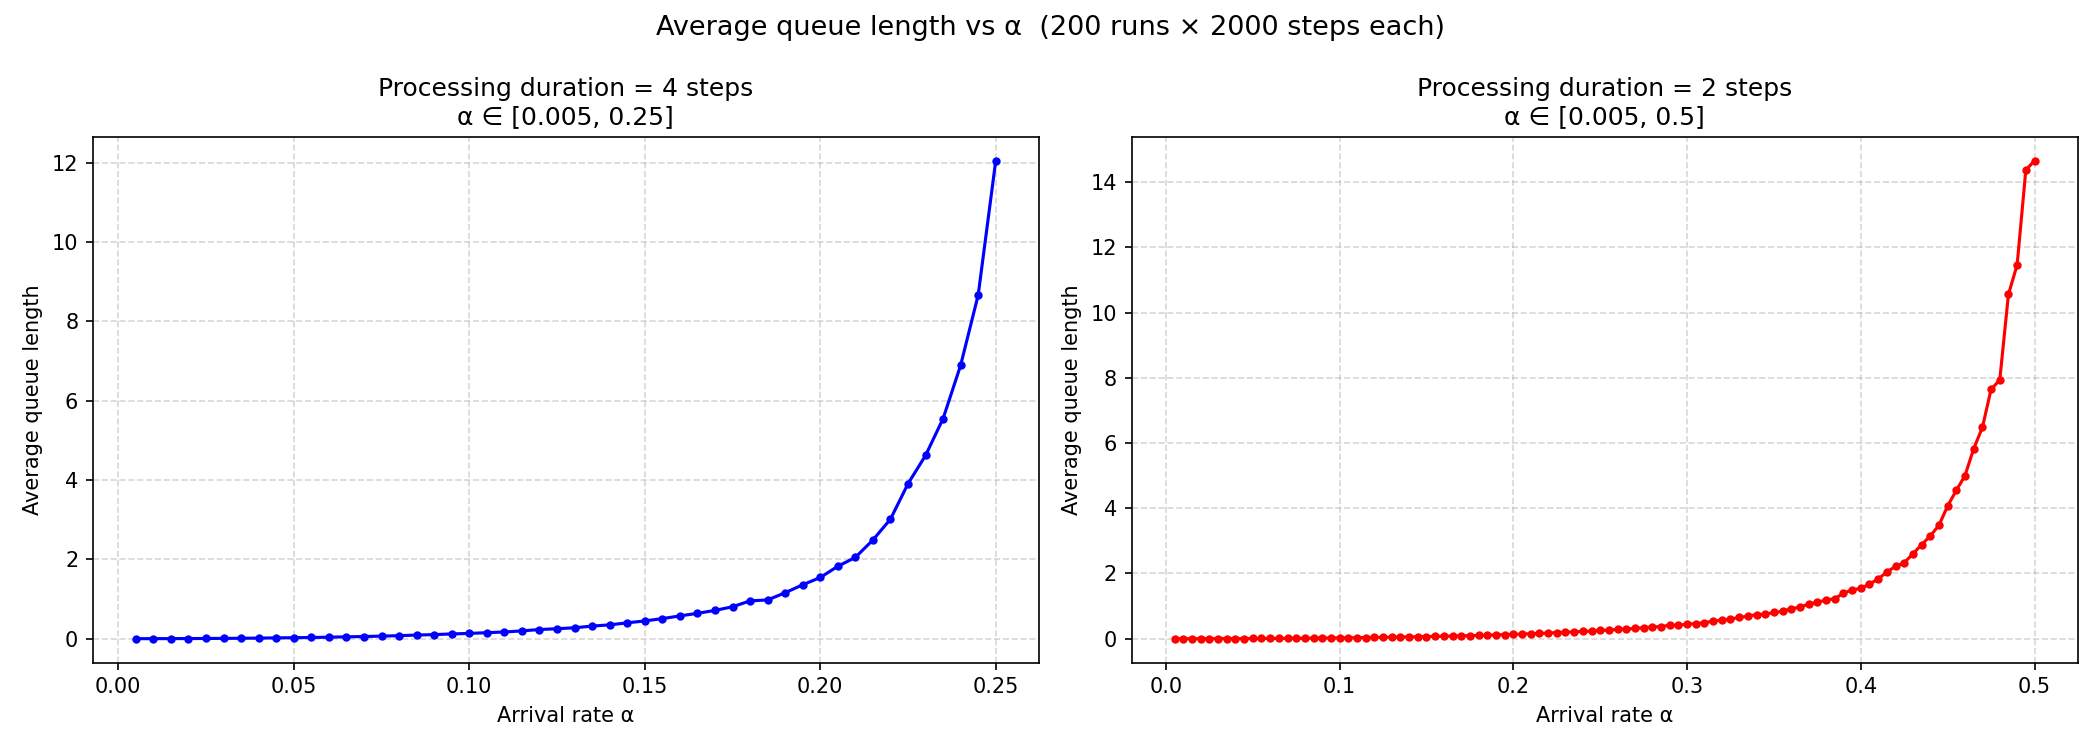
\includegraphics[width=\textwidth]{task_1/plots/task1e_comparison.png}
    \caption{Side-by-side comparison of average queue length vs.\ $\alpha$ for
             processing durations of 4 (left) and 2 (right) steps per job.}
    \label{fig:1e}
\end{figure}

\paragraph{Discussion.}
Halving the processing duration doubles the server throughput from 0.25 to
0.50 jobs/step.  Consequently the critical arrival rate at which the queue
explodes shifts from $0.25$ to $0.50$. This confirms that the saturation threshold is governed purely by the ratio
$\alpha / (1/\text{processing\_duration})$.

\newpage
% =============================================================================
\section{Task 2 -- Synchronization of a Swarm}
% =============================================================================

\subsection{Overview}

We simulate a population of $N = 150$ fireflies scattered uniformly in a
$1\times1$ square.  Each firefly has a clock of length $L = 50$ steps: it
flashes for the first $L/2 = 25$ steps and is dark for the remaining 25.
Fireflies interact locally: one step after starting to flash (i.e., at
\texttt{clock = 1}), a firefly checks its neighbours within radius $r$ and
applies a local majority rule -- if more than half of its neighbours
are currently flashing, it advances its own clock by an extra step, which
causes it to flash one step earlier in the next cycle.

\subsection{Implementation}

\paragraph{Firefly class (\texttt{firefly.py}).}
Each firefly stores its $(x, y)$ position (drawn from $\mathcal{U}[0,1]^2$
at creation), its current clock value, and the cycle length $L$.  Three
helper methods implement the task logic:

\begin{itemize}
    \item \texttt{is\_flashing()} -- returns \texttt{True} when
          \texttt{clock} $< L/2$.
    \item \texttt{should\_check\_neighbors()} -- returns \texttt{True} when
          \texttt{clock == 1} (one step after starting to flash).
    \item \texttt{corrects\_clock()} -- increments clock by 1 (correction step).
    \item \texttt{tick()} -- advances clock by 1 and wraps modulo $L$.
\end{itemize}

\paragraph{Simulation loop (\texttt{simulate\_2a.py}, \texttt{simulate\_2b.py}).}
Each time step proceeds in three phases:
\begin{enumerate}
    \item \textbf{Observation:} fireflies at \texttt{clock == 1} count their
          flashing neighbours within radius $r$; if a strict majority is
          flashing they are marked for correction.
    \item \textbf{Correction:} all marked fireflies call
          \texttt{corrects\_clock()}.
    \item \textbf{Tick:} all fireflies call \texttt{tick()}.
\end{enumerate}

\subsection{Subtask a -- Flashing Over Time for Different Radii}

Figure~\ref{fig:2a} shows the number of concurrently flashing fireflies over
5000 time steps for $r \in \{0.05, 0.1, 0.5, 1.4\}$.

\begin{figure}[h]
    \centering
    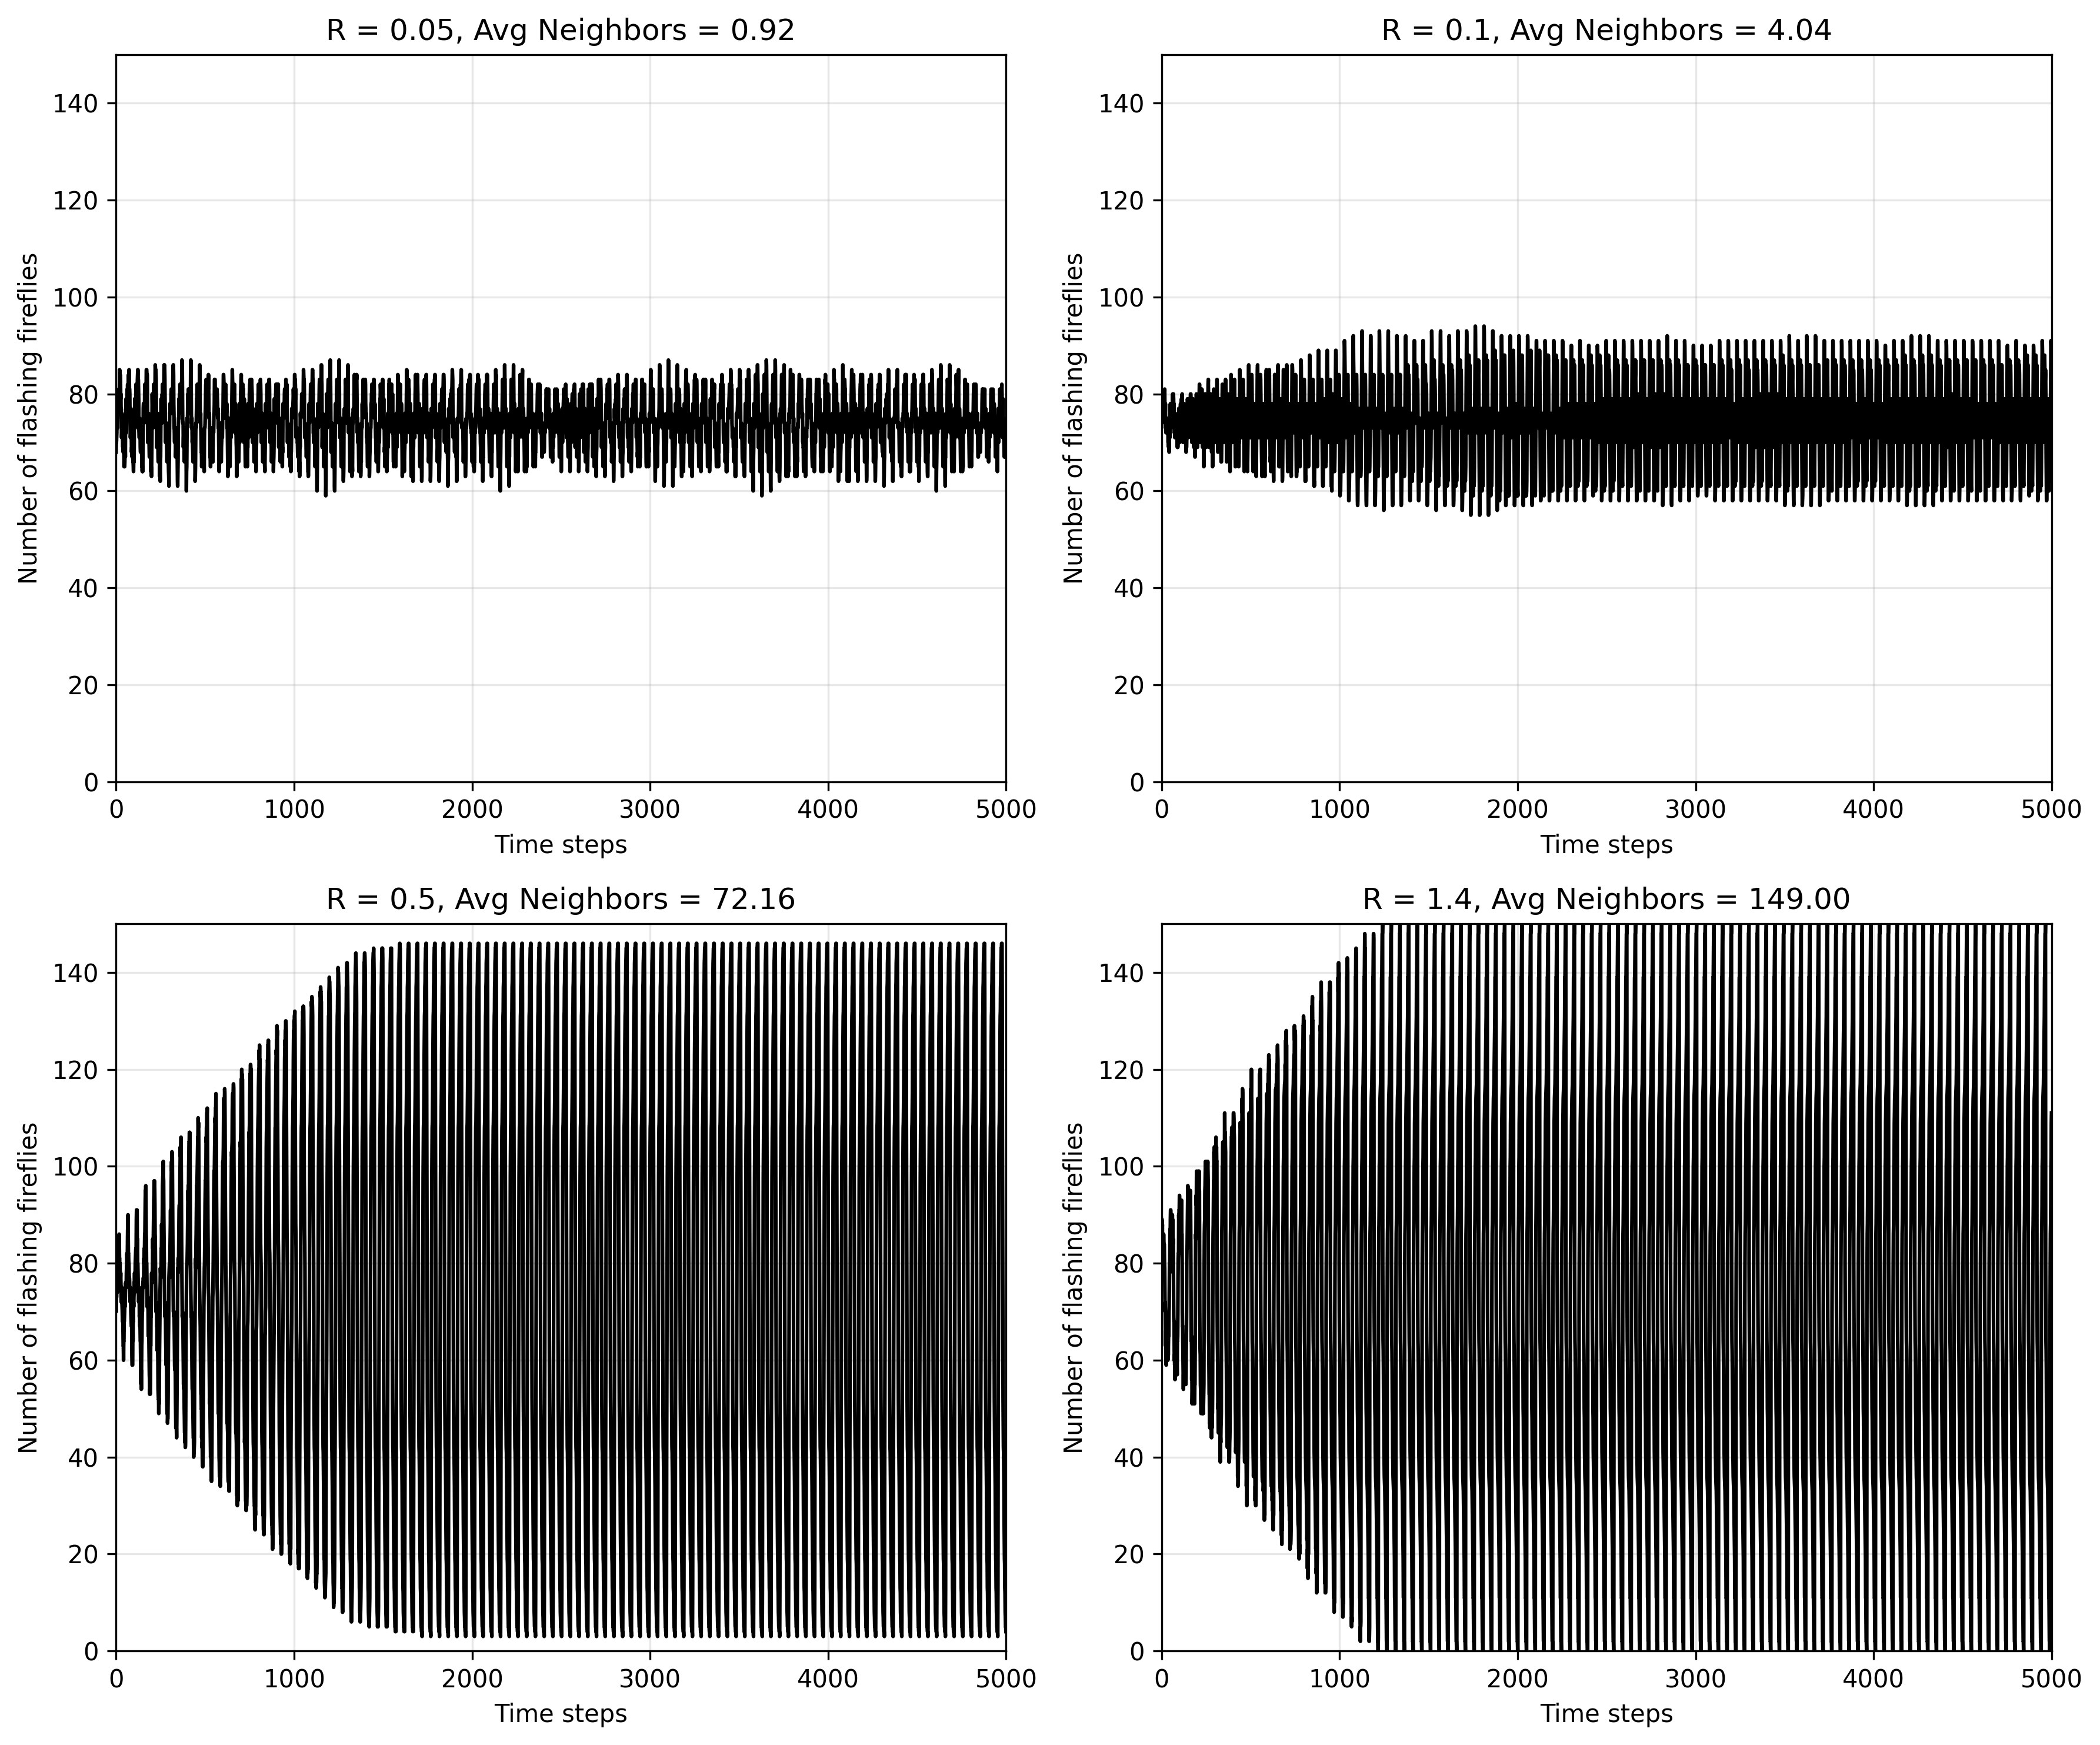
\includegraphics[width=\textwidth]{task_2/task2a_flashing_over_time.png}
    \caption{Number of flashing fireflies over time for four vicinity radii.
             $N = 150$, $L = 50$, 5000 time steps.}
    \label{fig:2a}
\end{figure}

\paragraph{Discussion.}

\begin{itemize}
    \item \textbf{$r = 0.05$ (avg.\ 0.92 neighbours):} Almost no connectivity.
          The count oscillates randomly around $N/2 = 75$ with no visible
          synchronization.
    \item \textbf{$r = 0.1$ (avg.\ 4.04 neighbours):} Still too sparse; weak
          local clustering but no global synchronization.
    \item \textbf{$r = 0.5$ (avg.\ 72 neighbours):} Clear synchronization
          emerges around $t \approx 1000$.  The population transitions to
          coherent oscillations between near-0 and near-150.
    \item \textbf{$r = 1.4$ (avg.\ 149 neighbours):} Nearly fully connected.
          Synchronization is fastest and most stable, with maximum amplitude.
\end{itemize}

A critical connectivity threshold lies between $r = 0.1$ and $r = 0.5$;
below it local interactions are insufficient to propagate phase corrections
across the swarm.

\subsection{Subtask b -- Synchronization Amplitude vs.\ Vicinity Radius}

The amplitude of the last cycle (last $L = 50$ steps) is defined as
$\max(\text{flashing}) - \min(\text{flashing})$.  We averaged this measure
over 50 independent simulation runs for each
$r \in [0.025,\,1.4]$ (step 0.025).  The result is shown in
Figure~\ref{fig:2b}.

\begin{figure}[h]
    \centering
    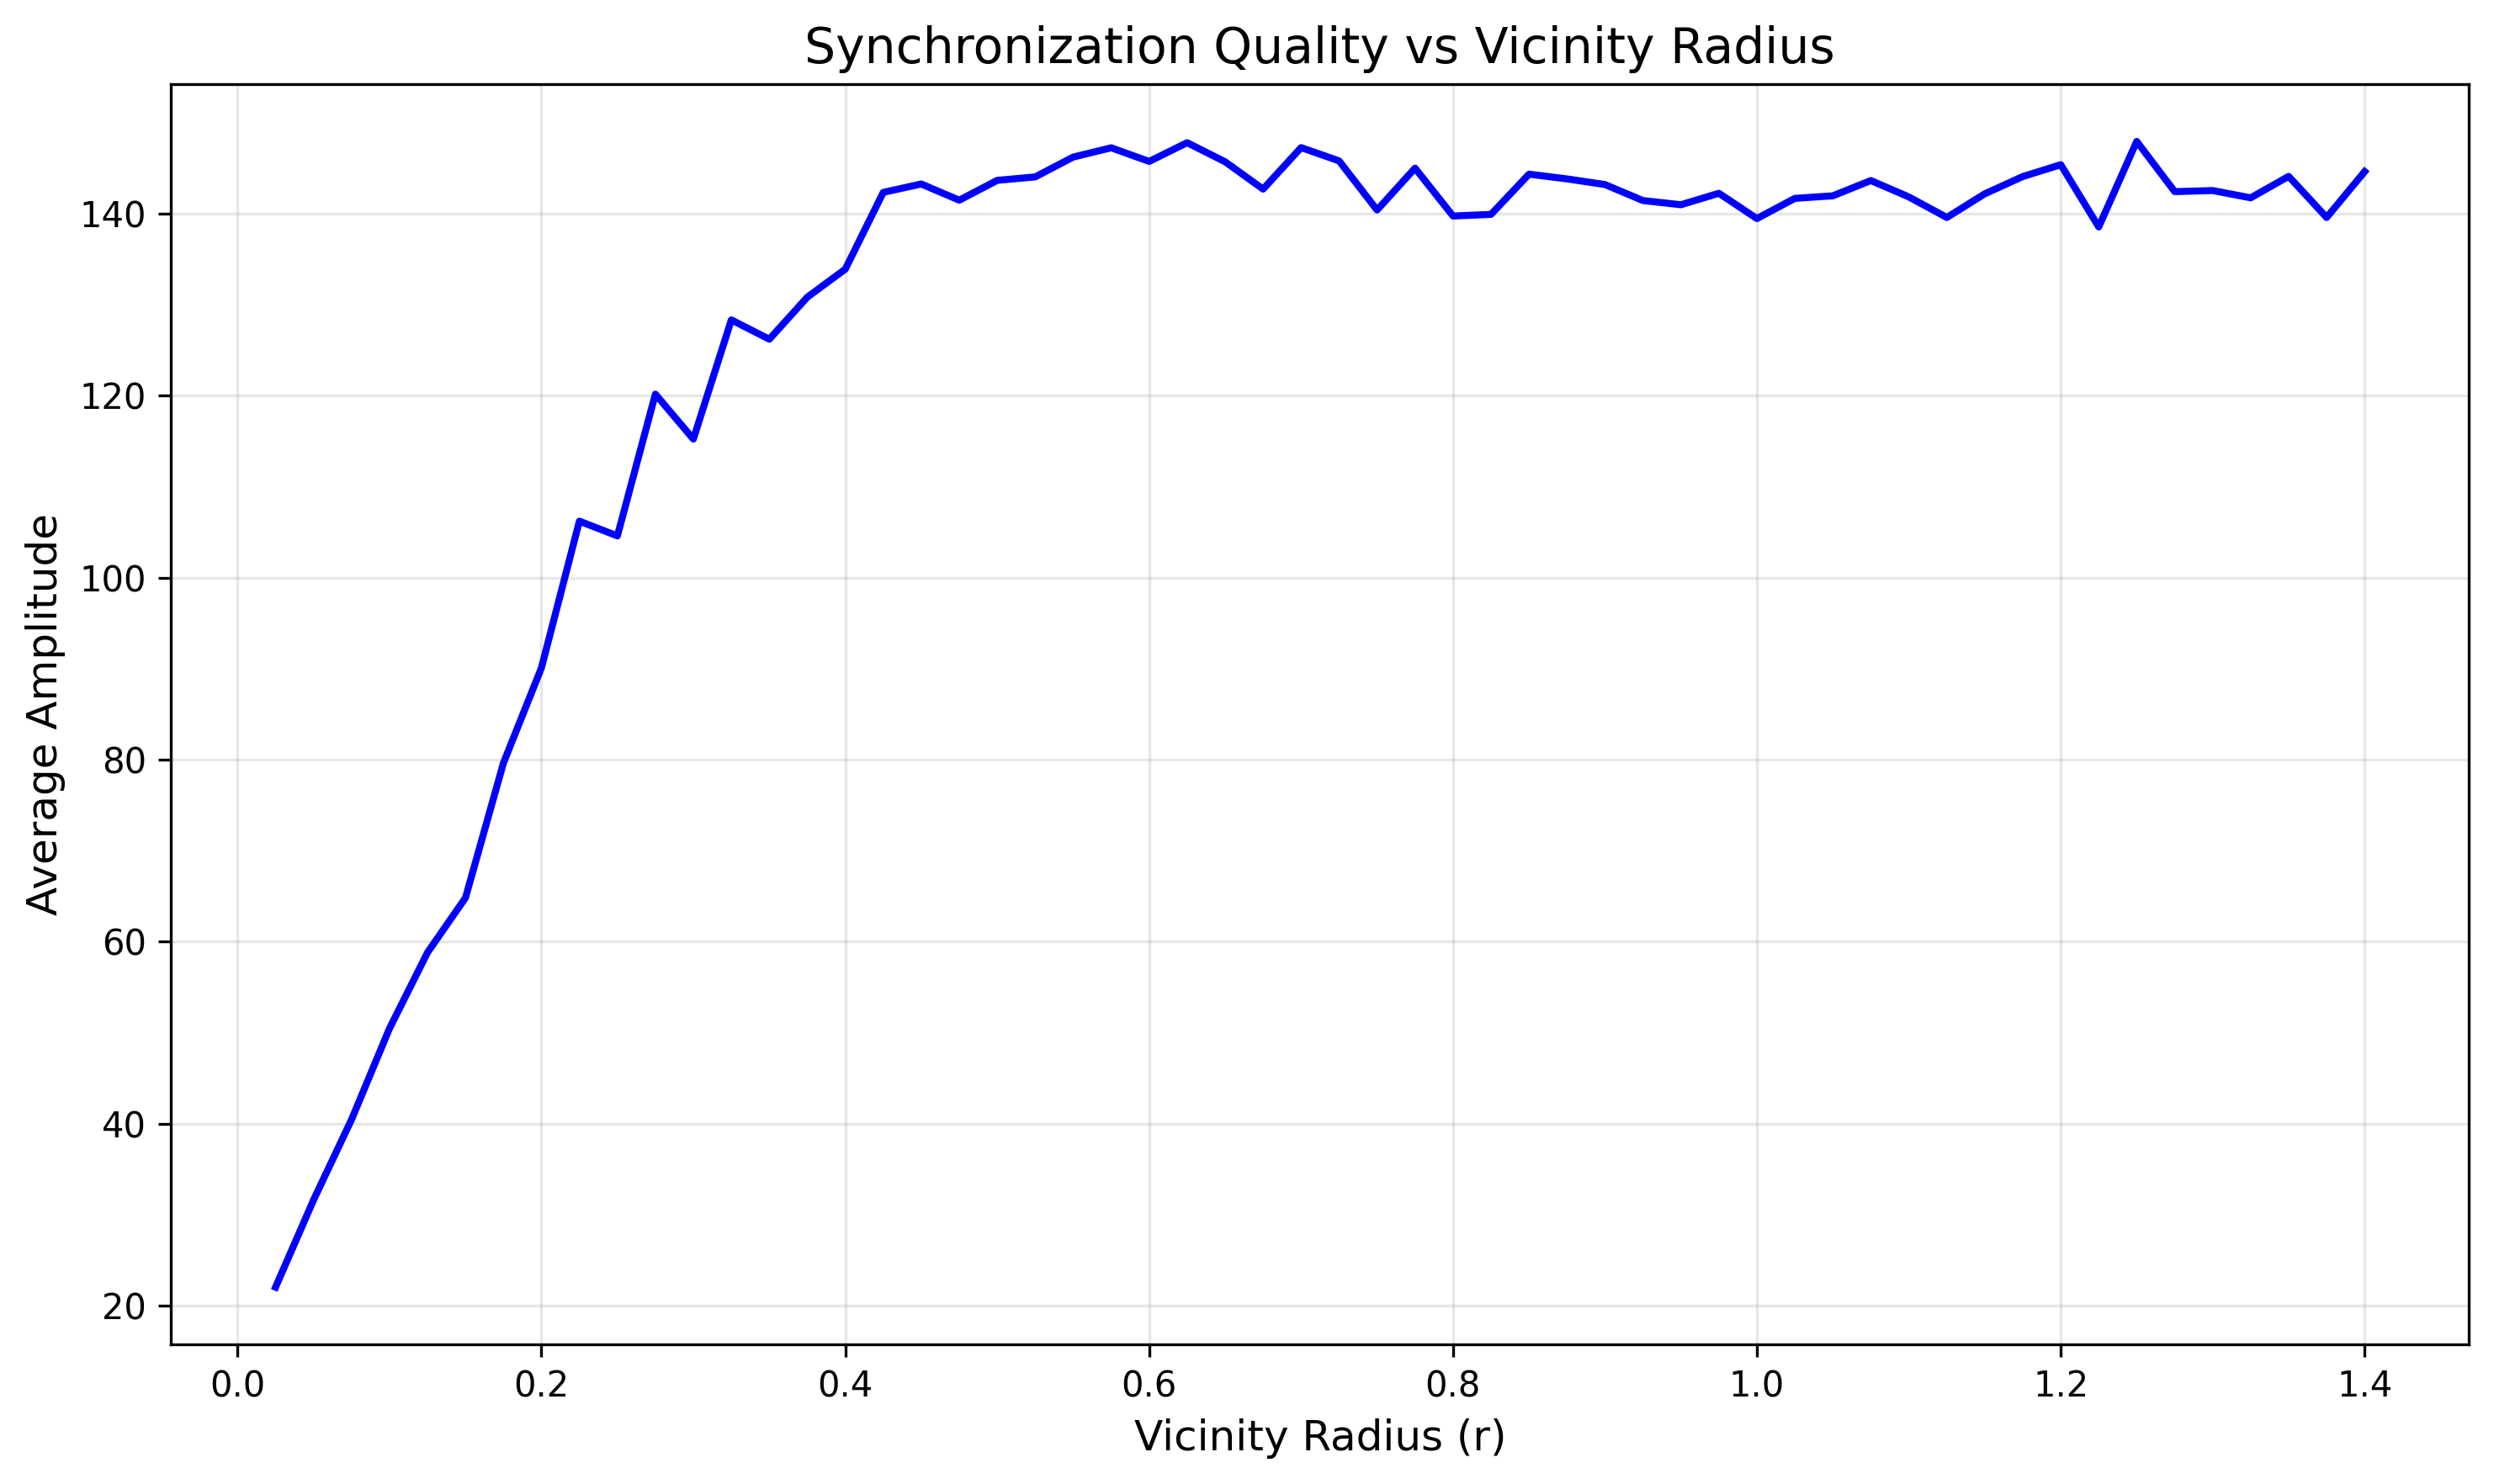
\includegraphics[width=0.85\textwidth]{task_2/task2b_amplitude_vs_radius.png}
    \caption{Average synchronization amplitude vs.\ vicinity radius $r$
             (50 runs $\times$ 5000 steps each).}
    \label{fig:2b}
\end{figure}

\paragraph{Discussion.}
Three regions are visible:

\begin{enumerate}
    \item \textbf{$r < 0.3$:} Amplitude rises steeply from $\approx 20$ to
          $\approx 100$.  Connectivity is insufficient for global sync; only
          small local clusters form.
    \item \textbf{$r \approx 0.3$--$0.5$:} Amplitude plateaus at its maximum
          ($\approx 140$--$148$).  This is the optimal operating range.
    \item \textbf{$r > 0.5$:} Amplitude remains high.  Additional connectivity
          does not improve synchronization -- diminishing returns.
\end{enumerate}

\paragraph{Good choice for vicinity and swarm density.}
For a swarm density of 150 fireflies in a $1\times1$ square, a vicinity radius
of $r \approx 0.3$--$0.4$ is optimal.  It provides enough neighbours
(${\sim}20$--$40$) for reliable majority voting while keeping the sensing
range small (energy-efficient, bio-plausible).

\paragraph{Interpretation of amplitude.}
A \emph{low amplitude} means fireflies flash nearly independently: at any
moment, roughly half the swarm flashes (${\sim}75$ out of 150), with no
coherent peaks.  A \emph{high amplitude} means the swarm flashes
collectively: almost all fireflies flash simultaneously, and the count swings
close to 0 and 150 each cycle.  Amplitude is therefore a direct measure of
\emph{synchronization quality}.

\newpage
% =============================================================================
\section{Completed Tasks}
% =============================================================================

\begin{center}
\begin{tabular}{lll}
\toprule
\textbf{Task} & \textbf{Description} & \textbf{Status} \\
\midrule
1a & Plot Poisson PMF for $\alpha \in \{0.01, 0.1, 0.5, 1\}$ & \checkmark \\
1b & Sampler from $P(X=i)$, empirical vs.\ theoretical plot    & \checkmark \\
1c & 2000-step simulation, $\alpha=0.1$, 4 steps/job           & \checkmark \\
1d & Avg.\ queue length vs.\ $\alpha \in [0.005, 0.25]$, 200 runs & \checkmark \\
1e & Comparison: 2-step vs.\ 4-step processing                 & \checkmark \\
\midrule
2a & Flashing over time for $r \in \{0.05, 0.1, 0.5, 1.4\}$   & \checkmark \\
2b & Amplitude vs.\ $r \in [0.025, 1.4]$, 50 runs              & \checkmark \\
\bottomrule
\end{tabular}
\end{center}

\end{document}
